% Exam package: Instructions & student name

\documentclass{exam}
\usepackage{graphicx}

\pagestyle{headandfoot}
\runningheader{Introduction to Information Technology}{}{Midterm}
\runningheadrule
\runningfooter{}{Page \thepage\ of \numpages}{}

% To hide points
% \nopointsinmargin
% \pointformat{}

\begin{document}
\addpoints

\begin{center}
    \vspace{2in}
    {\Large Introduction to Information Technology Midterm}
    \vspace{1.8in}

    \begin{figure}[h]
        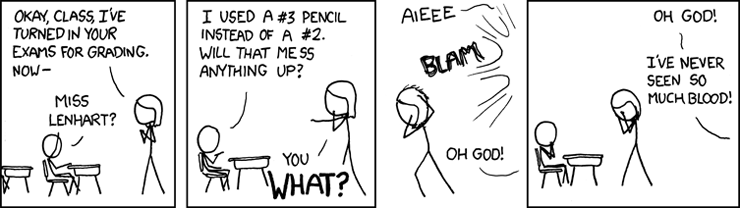
\includegraphics[width=\linewidth]{scantron.png}
    \end{figure}

    \vspace{1.3in}
    \fbox{\fbox{\parbox{5.5in}{\centering
            \textbf{Read carefully before starting the test:}
            \begin{itemize}
                \item Answer the questions using pencil or
                    a blue or black pen.
                \item You can use a calculator if you want, but it can't have internet access.
                \item Answer the questions in the spaces provided on the
                question sheets. If you run out of room for an answer,
                continue on the back of the page
                \item You are allowed one sheet 11.5 x 8in paper (or smaller) of handwritten notes
            \end{itemize}}}}

\vspace{0.2in}
\end{center}

\makebox[\textwidth]{\textsc{Full name:}\enspace\hrulefill}

\vspace{0.2in}

\makebox[\textwidth]{\textsc{Computing ID:}\enspace\hrulefill}

\vspace{0.2in}
\gradetable[h][pages]
\newpage

\begin{questions}
\section{True or False (10 Points)}
\question[1] T / F : A digital signal has a limited precision. 
\question[1] T / F : Solid State Drives use a spinning disk to read and write information.
\question[1] T / F : Boolean logic is the basis of computer circuit design.
\question[1] T / F : LAN networks typically use WiFi to wireless transport information.
\question[1] T / F : Programming Languages can tell computers to do things binary programs can't. 
\question[1] T / F : Network packets can be sent independently of each other in parallel.
\question[1] T / F : Software as a Service (SaaS) is the most general form of cloud computing
\question[1] T / F : CSS can change the way HTML is displayed on a browser.
\question[1] T / F : Stochastic Gradient Descent is a method to train machine learning models.
\question[1] T / F : An overfit machine learning model will perform poorly on the training set.

\section{Multiple Choice (10 Points)}
\question[1] Which of the following does not have the primary task of performing computation?
\begin{choices}
    \choice The GPU
    \choice The Motherboard
    \choice The CPU
    \choice All of the above
\end{choices}
\question[1] Which of the following is a constant in boolean logic:
\begin{choices}
    \choice $\oplus$
    \choice X
    \choice And
    \choice True
\end{choices}
\question[1] The Internet Protocol Suite layer which defines where information is sent is:
\begin{choices}
    \choice The Internet Layer
    \choice The Link Layer
    \choice The Application Layer
    \choice The Transport Layer
\end{choices}
\question[1] Which core language of the internet is mainly responsible for dynamic content:
\begin{choices}
    \choice HTML
    \choice Javascript
    \choice CSS
    \choice Emerald
\end{choices}

\newpage
\question[1] Which component of the Model-View-Controller pattern is responsible for maintaining a database: 
\begin{choices}
    \choice The View
    \choice The Model
    \choice The Controller
    \choice All of the above
\end{choices}

\question[1] Which is not a class of learning in machine learning:
\begin{choices}
    \choice Supervised Learning
    \choice Reinforcement Learning
    \choice Chaos Learning
    \choice Unsupervised Learning
\end{choices}
\question[1] Which of the following is a component of a computer's CPU (Central Processing Unit)?
\begin{choices}
    \choice Hard Drive
    \choice RAM (Random Access Memory)
    \choice Graphics Card
    \choice ALU (Arithmetic Logic Unit)
\end{choices}
\question[1] Spreadsheet formulas can include: 
\begin{choices}
    \choice Cell references
    \choice Hard coded Values
    \choice Functions
    \choice All of the Above
\end{choices}
\question[1] Database Management Systems include
\begin{choices}
    \choice A physical device to store data
    \choice A way to store, access, and update data
    \choice Developers that maintain the database
    \choice A general purpose programming language
\end{choices}
\question[1] In a database, the field responsible for uniquely identifying a data point is the 
\begin{choices}
    \choice Primary Key
    \choice Primary Field
    \choice Unique Key
    \choice Unique Field
\end{choices}

\bonusquestion[1] What town is Will from? (I told you it would be on the test) 
\begin{choices}
    \choice Oak Forest, IL
    \choice Peoria, IL
    \choice Tinley Park, IL
    \choice Lincoln, NE
\end{choices}

\newpage
\section{Show Your Work (21 Points)}
\question[3] Convert 242 to binary:
\vspace{4.5in}
\question[3] Convert 10011011 to decimal:
\newpage 

\question[5] Produce the truth table for the following logical expression:
\[
X \land Y \rightarrow \lnot(X \lor Z)
\]
\vspace{4in}

\question[5] Is $\lnot (P \land Q)$ logically equivalent to $(\lnot P) \lor (\lnot Q)$? Show why or why not and explain:

\newpage
\question[5] The following network has been trained to predict how many peppers will grow on a plant by September based on the hardiness zone and month it was planted in. I'm going to plant my peppers in Charlottesville (zone 7) in April (month 4). Using this network, calculate the value of each neuron based on how I'm planting my pepper plant and tell me how many peppers I should expect based on the network's output.

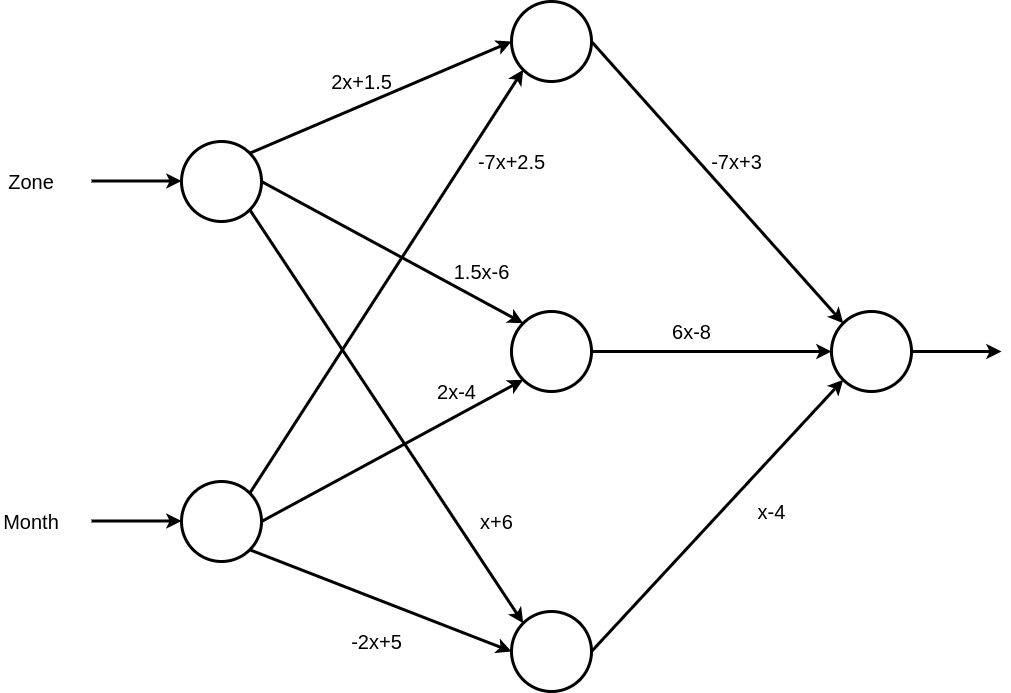
\includegraphics[width=\linewidth]{network.png}

\newpage

\section{Short Answer (19 Points)}
\question[3] What is the importance of binary in computing?
\vspace{2in}

\question[3] Why was the world wide web important to the spread of the internet?
\vspace{2in}

\question[4] What is the difference between Personal Area Networks (PAN) and Local Area Networks? List two devices that would connect to a PAN and two that would connect to a LAN.
\vspace{2in}

\question[3] Describe two benefits of cloud computing:
\newpage

\question[3] Explain the purpose of the frontend and backend in website architecture:
\vspace{2in}

\question[3] When we say a model ``learns'' in machine learning, what do we mean?
\vspace{2in}


\bonusquestion[2] One of the multiple choice questions was generated by a transformer model. Pick which question you think it was and explain. (1 point for choosing the right question and 1 point for your explanation. You don't have to choose the right one to get the second point. Just explain your reasoning based on our discussions of machine learning.)
\end{questions}

\end{document}